\chapter{Sintesi dell'Anidride Maleica}

\section{Caratteristiche chimico-fisiche}
Temperatura di fusione = 53�C (326.1K)\\
Temperatura di normal ebollizione = 202�C (475.1K)

\section{Principali impieghi}
L'\textit{anidride maleica} viene prodotta nei quantitativi riportati in \tablename~\ref{tab:AM:WorldProduction}, e i principali utilizzi sono la realizzazione di \textit{resine poliestere insature} (a cui finisce il 40-60\% della produzione) e la realizzazione di \textit{acido maleico} e \textit{fumarico} (10 - 15\% della produzione); il restante viene impiegato come materia prima per i processi della chimica secondaria, in particolare per la realizzazione di pesticidi, plastificanti o additivi per lubrificanti.

\begin{table}
	\centering
		\begin{tabular}{lccc} \hline
													& 1990		& 1992		& 1995		\\ \hline
			USA									& 0.193		& 0.193		& 0.251		\\
			Europa occidentale	& 0.200		& 0.175		& 0.188		\\
			Giappone						& 0.101		& 0.104		& 0.113		\\ \hline
		\end{tabular}
	\caption[Produzione mondiale di \textit{anidride maleica} dal 1990 al 1995 ]{Produzione mondiale di \textit{anidride maleica} nel periodo 1990 - 1995 nelle varie zone del mondo ($\times10^6$ tonn/anno)}
	\label{tab:AM:WorldProduction}
\end{table}

La reazione di idratazione dell'anidride per passare ad acido maleico � reversibile, ma se l'acido maleico viene riscaldato si ha isomerizzazione che porta alla formazione di acido fumarico, che non pu� pi� essere trasformato in anidride maleica (\figurename\ref{rxn:AM:IdratIsomerizAM}). L'isomerizzazione avviene a circa 100�C.
\begin{figure}
	\centering
		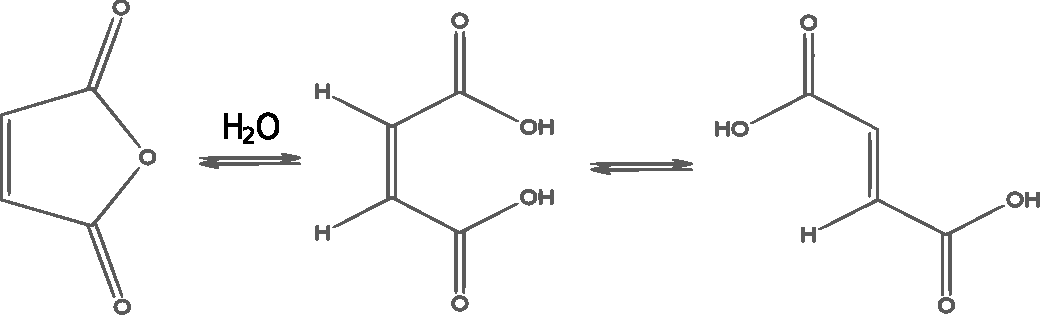
\includegraphics[width=0.60\textwidth]{image/IdratIsomerizAM.pdf}
	\caption{Reazione di idratazione dell'\textit{anidride maleica} per dare \textit{acido maleico} e sua isomerizzazione per dare \textit{acido fumarico}.}
	\label{rxn:AM:IdratIsomerizAM}
\end{figure}

Il processo produttivo utilizzato fino ai primi anni '60 comportava l'ossidazione del benzene, ma successivamente si � preferito optare per il processo di ossidazione di idrocarburi $C_4$ (principalmente \textit{n-butano} ma anche n-butene con alto tenore paraffinico). Attualmente il processo da butano copre il 60\% della produzione mondiale di anidride maleica.

\section{Processo da BENZENE}

\subsection{Reazione principale}
Il processo per la produzione di anidride maleica a partire da benzene � un'ossidazione particolarmente esotermica, accompagnata da un processo di combustione, come � evidente dalla reazione \ref{rxn:AM:ProduzAMDaBenzene}
\begin{equation}
	C_6H_6 + \frac{9}{2} O_2 \rightarrow C_4H_2O_3 + 2 H_2O + 2 CO_2
	\label{rxn:AM:ProduzAMDaBenzene}
\end{equation}
Il cui $\Delta H^o$ � di -447 Kcal/mol. La reazione avviene in presenza di un catalizzatore composto da pentossido di vanadio ($V_2O_5$) e ossido di molibdeno ($MoO_3$) attivati da acido fosforico e supportati su $\alpha-Al_2O_3$.

\subsection{Condizioni operative}
La reazione viene condotta a temperature comprese tra 350 e 400�C a pressioni di 1 - 5Bar. I tempi di contatto tra i reagenti e il catalizzatore all'interno del reattore sono di circa un decimo di secondo ($\tau = 0.1s$) e si utilizza un forte eccesso di aria per far si di essere al di sotto del limite di infiammabilit� della miscela benzene - aria (LI = 1.4\% v/v).

La resa di conversione del benzene per passaggio � del 85 - 95\%, con una selettivit� verso la formazione dell'anidride maleica $\leq 75\%$; inoltre se si cerca di aumentare la resa per passaggio del benzene si ha una diminuzione della selettivit�. Lo sviluppo di calore � di circa 7000 kcal/kg di benzene convertito, quindi si ha un'elevata quantit� di calore da sottrarre.

\subsection{Reattore ed impianto}
Il reattore � costituito da una serie di tubi (fino a 13000) del diametro da 1 pollice (2.54cm) al cui interno si trova il catalizzatore. Il reattore pu� avere un diametro massimo di 4.5m. All'esterno delle tubature si trova un bagno di sali fusi (una miscela di $KNO_3$ e $NaNO_3$ in rapporto 57:43) che vengono poi utilizzati per produrre vapore ad alta pressione. Non � possibile utilizzare direttamente acqua bollente per raffreddare il reattore inquanto ci si trova in condizioni vicine alle condizioni critiche dell'acqua e di conseguenza il $\Delta H_{ev}$ sarebbe troppo basso per assorbire tutto il calore liberato. L'utilizzo di sali permette un controllo della temperatura molto accurato ($\pm 0.5^oC$)

L'impianto prosegue con un condensatore, che abbassa la temperatura dei gas in uscita al di sotto della temperatura di condensazione dell'\textit{anidride maleica}, che viene cos� separata, mentre i gas non condensati (contenenti ancora una discreta quantit� del prodotto) vengono raffreddati con acqua che abbatte anche l'anidride maleica rimanente sotto forma di \textit{acido maleico}. L'\textit{acido maleico} viene concentrato e disidratato per dare anidride maleica che viene ulteriormente purificata per mezzo di una distillazione (dalla cui teste esce \textit{AM} al 99.5\%)

Gli svantaggi dovuti all'utilizzo di questo processo produttivo sono dovuti al fatto di utilizzare una materia prima costosa (il benzene viene ottenuto dallo \textit{steam cracking} del petrolio e dal topping dei grezzi aromatici) e molto tossica (cancerogena) con tutte le problematiche di sicurezza che ne derivano. Infine si ha una perdita di due atomi di carbonio per ogni anello aromatico reagito per dare \textit{anidride maleica}.

\section{Processo da BUTANO}

Il processo da butano fu sviluppato a partire dal 1974 dalla Monsanto inquanto permette di utilizzare un reagente meno costoso e pericoloso del benzene, inoltre evita l'inutile ossidazione di 2 atomi carbonio e di conseguenza un minor sviluppo di calore da smaltire.

\subsection{Reazione principale}
La reazione complessiva di sintesi dell'\textit{anidride maleica} a partire dall'\textit{n-butano} � riassunta in \ref{rxn:AM:ProduzAMDaButano}
\begin{equation}
	C_4H_10 + \frac{7}{2} O_2 \rightarrow C_4H_2O_3 + 2 H_2O
	\label{rxn:AM:ProduzAMDaButano}
\end{equation}
Il cui $\Delta H^o$ � di -335 Kcal/mol (quindi meno esotermica del processo da benzene). La reazione avviene in presenza di un catalizzatore composto da \textit{ossidi di vanadio} e promosso da \textit{fosforo} e ossidi di \textit{Fe}, \textit{Cr}, \textit{Ti}, \textit{Ni}, \textit{Co} e \textit{Mo}. 

Il catalizzatore ha il compito di effettuare una deidrogenazione ossidativa del butano a \textit{2-butene} (che viene adsorbito sul catalizzatore) e successivamente di favorire l'ossidazione dei gruppi metilici terminali (assicurato dal complesso \textit{V-P-O}).

\subsection{Reattori a letto fisso}
I primi impianti utilizzavano un reattore a letto fisso in cui far avvenire la reazione, inviando una miscela etilene - aria al di sotto dei limiti di infiammabilit� (1.8\% v/v) e operando a temperaure di 400 - 450�C. In uscita si ha una bassa concentrazione dell'\textit{AM} e di conseguenza � necesasrio convertire l'\textit{acido maleico} ad anidride nella fase successiva, con elevati costi di esercizio.

La conversione � dell'80\% del butano inviato al reattore e la selettivit� verso la produzione dell'anidride maleica � del 70\% circa; il butano non reagito viene bruciato per produrre il calore necessario all'impianto.

\subsection{Reattori a letto fluido}
In un secondo momento si ha la realizzazione di impianti in cui il reattore opera a letto fluido, migliorando lo smaltimento del calore. A causa degli elevati volumi necessari, per�, si � scelto di operare con una miscela pi� ricca in etilene (circa 4\% v/v) che pur rientrando nei limiti di esplosivit� della miscela permette di limitare i voumi e i costi di realizzazione. In questo modo in uscita si ha una concentrazione di \textit{anidride maleica} pi� elevata che riduce, anche, le successive spese di disidratazione e concentrazione dell'\textit{acido maleico}. Per limitare i rischi di esplosione si inserisce nella camera di reazione un terzo corpo (catalizzatore) che favorisce le reazioni di terminazione (impedendo cos� il propagarsi dell'esplosione).

Di contro si ha un fenomeno di erosione del catalizzatore che si muove all'interno del reattore e retromiscelazione dei gas. La conversione per passaggio � superiore all' 80\% del butano e la selettivit� verso anidride maleica � compresa tra il 50 e il 60\%. Il butano non reagito pu� essere riciclato per ridurre i costi di produzione.

\section{Processo ALMA}
Negli ultimi anni si � sviluppato il processo ALMA (\textbf{A}lusuisse Italia \textbf{L}ummus Crest \textbf{M}aleic \textbf{A}nhydride) che utilizza un particolare solvente brevettato per la separazione dell'anidride maleica che riduce i costi di investimento iniziali e le perdite di prodotto dei processi in cui l'assorbimento � in acqua (con successiva disidratazione). Lo schema dell'impianto � visibile in \figurename~\ref{fig:AM:SchemaALMA}, ove � evidente la parte iniziale in cui avviene la reazione, la successiva fase di separazione del prodotto e il recupero (e purificazione) del solvente per minimizzarne le perdite con infine una sezione per la purificazione dell'\textit{anidride maleica}.
\begin{figure}[htbp]
	\centering
		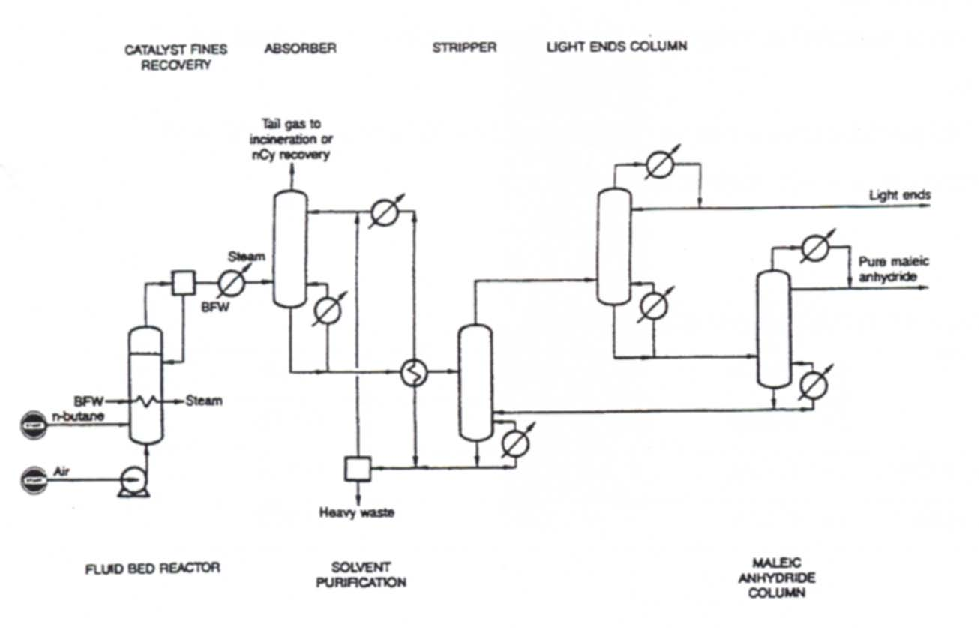
\includegraphics[width=0.80\textwidth]{image/AMSchemaALMA.pdf}
	\caption{Schema dell'impianto per la sintesi dell'\textit{anidride maleica} secondo il processo \textit{ALMA}}
	\label{fig:AM:SchemaALMA}
\end{figure}
